\documentclass[linenumbers]{aastex701}

% Every number below is a macro generated from research/results/atlas/ by
% research/figures/rnaas_atlas.py (written to research/results/rnaas_atlas/numbers.tex).
% GENERATED by research/figures/rnaas_atlas.py -- do not edit
\newcommand{\MayOnset}{10 May 2024, 15:00~UT}
\newcommand{\MayNSets}{2{,}294{,}139}
\newcommand{\MayNPrimary}{2{,}657}
\newcommand{\MayNPayload}{3{,}484}
\newcommand{\MayNQuiet}{8}
\newcommand{\MayPeakMin}{3.2}
\newcommand{\MayPeakMax}{5.4}
\newcommand{\MayNShells}{5}
\newcommand{\MayPeakFour}{3.2}
\newcommand{\MayLagFour}{9}
\newcommand{\MayPeakFourFifty}{3.8}
\newcommand{\MayLagFourFifty}{9}
\newcommand{\MayPeakFive}{4.0}
\newcommand{\MayLagFive}{9}
\newcommand{\MayPeakFiveFifty}{4.9}
\newcommand{\MayLagFiveFifty}{9}
\newcommand{\MayPeakSix}{5.4}
\newcommand{\MayLagSix}{9}
\newcommand{\MayLags}{9}
\newcommand{\MayRho}{1.00}
\newcommand{\MayHAOne}{passed}
\newcommand{\MayHATwo}{passed}
\newcommand{\MayHAThree}{passed}
\newcommand{\MayHAFour}{failed}
\newcommand{\MayDetectFrac}{100}
\newcommand{\MayDetectN}{4}
\newcommand{\MayConstMaxRatio}{2.3}
\newcommand{\MayNConst}{1{,}574}
\newcommand{\OctOnset}{10 October 2024, 15:00~UT}
\newcommand{\OctNSets}{1{,}815{,}748}
\newcommand{\OctNPrimary}{3{,}776}
\newcommand{\OctNPayload}{3{,}687}
\newcommand{\OctNQuiet}{8}
\newcommand{\OctPeakMin}{1.8}
\newcommand{\OctPeakMax}{2.7}
\newcommand{\OctNShells}{5}
\newcommand{\OctPeakFour}{1.8}
\newcommand{\OctLagFour}{9}
\newcommand{\OctPeakFourFifty}{2.1}
\newcommand{\OctLagFourFifty}{-3}
\newcommand{\OctPeakFive}{2.4}
\newcommand{\OctLagFive}{-3}
\newcommand{\OctPeakFiveFifty}{2.7}
\newcommand{\OctLagFiveFifty}{-3}
\newcommand{\OctPeakSix}{2.7}
\newcommand{\OctLagSix}{-3}
\newcommand{\OctLags}{-3, 9}
\newcommand{\OctRho}{1.00}
\newcommand{\OctHAOne}{failed}
\newcommand{\OctHATwo}{passed}
\newcommand{\OctHAThree}{passed}
\newcommand{\OctHAFour}{failed}
\newcommand{\OctDetectFrac}{100}
\newcommand{\OctDetectN}{4}
\newcommand{\OctConstMaxRatio}{2.0}
\newcommand{\OctNConst}{1{,}448}

\begin{document}

\title{Storm Drag on Tracked Debris, Shell by Shell: A Preregistered Look at the May and October 2024 Geomagnetic Storms}

\author[0009-0001-8293-8064]{Joyce Malik}
\affiliation{Department of Computer Science and Engineering, Dr. Ambedkar Institute of Technology, Bengaluru, India}
\email[show]{colossus@drait.edu.in}

\begin{abstract}
Geomagnetic storms heat the thermosphere, so objects in low Earth orbit lose altitude faster. We measure this from public orbital elements of uncontrolled debris and rocket bodies, which cannot manoeuvre and so act as passive drag probes. For each 50\,km altitude shell, we take the median ratio of an object's decay rate to its own quiet-time rate. All definitions and hypotheses were committed before the data were downloaded. In the May 2024 storm, the ratio peaked at \MayPeakMin--\MayPeakMax{} times quiet levels, \MayLagFour\,h after onset, and rose steadily with altitude. The October 2024 storm reproduced the altitude trend at lower peaks (\OctPeakMin--\OctPeakMax), but failed the preregistered timing test. Payload samples gave larger peaks than debris in both storms, so station-keeping satellites should be kept out of such measurements.
\end{abstract}

\section{Why debris}
When the thermosphere heats up during a storm, its density at a fixed altitude goes up, and so does the drag on everything orbiting there. Debris and spent rocket bodies are useful here because they never fire thrusters, so any change in how fast they decay comes from the atmosphere. Deriving thermospheric density from the decay of tracked debris is an established idea \citep{Johlander2026,Constant2024}. What we add is small and specific: a preregistered, shell-resolved comparison of two storms, with the failed tests reported, and a direct check of how much payloads distort such a measurement.

\section{Data and method}
We used Space-Track (\url{https://www.space-track.org}) \texttt{gp\_history} element sets for near-circular objects below about 1000\,km, object types from the CelesTrak SATCAT (\url{https://celestrak.org}), and the GFZ Potsdam Kp index \citep{Matzka2021,Matzka2021data}. The May window has \MayNSets{} element sets and the October window \OctNSets.

The semi-major axis comes from the mean motion, and an object's decay rate is the change in semi-major axis between consecutive element sets 0.2--2\,d apart, binned to 12\,h. Each object's quiet rate is its median over \MayNQuiet{} quiet days before the storm (daily maximum Kp $\leq 4$). Objects that are not clearly drag-dominated are dropped. The storm ratio of an object is its rate divided by its quiet rate, so it tracks density relative to quiet conditions with no density model needed. For each shell and time bin, we take the median ratio over at least 30 objects. The primary sample is debris and rocket bodies (\MayNPrimary{} objects in May, \OctNPrimary{} in October). Payloads are kept separate and never merged in.

The preregistration fixed four hypotheses. HA1 says every shell from 350 to 550\,km peaks within 0--72\,h of onset, the first 3-hour Kp of at least 7. HA2 says the peak ratio rises with altitude (Spearman $\rho > 0$). HA3 says the peak clears the quiet mean plus five standard deviations in at least 80\% of shells. HA4 says payloads do not peak higher than debris. The October run was a separate replication preregistration with the same definitions, committed before its data were fetched.

\section{Results}
In May (onset \MayOnset), the ratio peaked in every shell \MayLagFour\,h after onset, from \MayPeakFour{} at 400\,km to \MayPeakSix{} at 600\,km (Figure~\ref{fig:atlas}). HA1 \MayHAOne, HA2 \MayHATwo{} ($\rho = \MayRho$ over \MayNShells{} shells) and HA3 \MayHAThree{} (\MayDetectFrac\% of \MayDetectN{} shells), but HA4 \MayHAFour.

October (onset \OctOnset) was a weaker storm for drag, with peaks from \OctPeakFour{} at 400\,km to \OctPeakSix{} at 600\,km. The altitude trend held (HA2 \OctHATwo, $\rho = \OctRho$) and so did detectability (HA3 \OctHAThree), but HA1 \OctHAOne. Shells from 450\,km upward peaked in the 12\,h bin that contains the onset, and that bin starts 3\,h before it, so their lag counts as negative. With 12\,h bins, the timing test as we wrote it cannot tell a prompt response from an early one. We report the failure as preregistered and did not change the rule.

HA4 \OctHAFour{} again, and this one matters. Payloads include satellites that hold their altitude with thrusters, and their peaks were larger, not smaller. In October we tested this directly. Constellation satellites (\OctNConst{} objects) peaked above debris in every shell, up to \OctConstMaxRatio{} times higher, while other payloads stayed within 0.8--1.25 times the debris peak. So a catalogue-wide decay measurement that includes manoeuvring satellites will overstate storm drag. That is why the debris-only sample is the one to trust.

\begin{figure}[h]
\centering
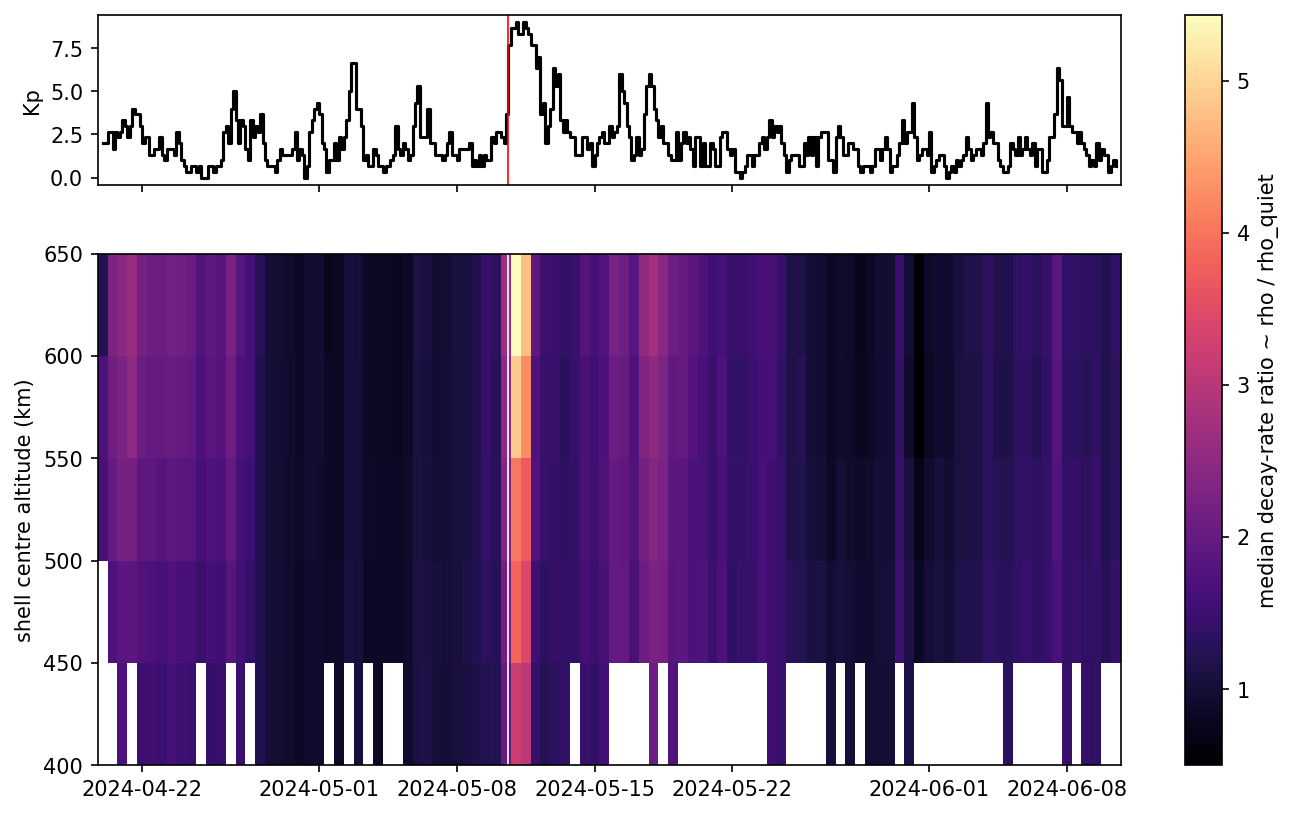
\includegraphics[width=\columnwidth]{atlas_primary.png}
\caption{May 2024. Top: Kp, with the onset marked. Bottom: median decay-rate ratio of debris and rocket bodies (a proxy for density relative to quiet conditions), by altitude shell and 12\,h bin. White cells have fewer than 30 objects.}
\label{fig:atlas}
\end{figure}

\section{Limits}
Mean-element semi-major axes carry noise of tens of metres. Our time resolution is 12\,h, solar flux is not regressed out, and the ratio is a relative proxy that we have not compared with an independent density model. The result is a known effect, measured cleanly for the whole public catalogue, not new physics.

\section*{Data and code}
Code, preregistrations and every output: \url{https://github.com/joycemalik/orbitalnet-dashboard} (\texttt{research/atlas/}, \texttt{research/results/atlas/}). Space-Track data are not redistributed.

\software{NumPy \citep{Harris2020}, pandas \citep{McKinney2010}, SciPy \citep{Virtanen2020}, Matplotlib \citep{Hunter2007}}

\begin{thebibliography}{}
\bibitem[Constant et al.(2024)]{Constant2024} Constant, C., et al. 2024, arXiv:2408.16805
\bibitem[Harris et al.(2020)]{Harris2020} Harris, C.~R., et al. 2020, Natur, 585, 357
\bibitem[Hunter(2007)]{Hunter2007} Hunter, J.~D. 2007, CSE, 9, 90
\bibitem[Johlander et al.(2026)]{Johlander2026} Johlander, A., Papadogiannakis, A., \& Rasmusson, J. 2026, JSWSC, 16, 7
\bibitem[Matzka et al.(2021a)]{Matzka2021} Matzka, J., Stolle, C., Yamazaki, Y., Bronkalla, O., \& Morschhauser, A. 2021, SpWea, 19, e2020SW002641
\bibitem[Matzka et al.(2021b)]{Matzka2021data} Matzka, J., Bronkalla, O., Tornow, K., Elger, K., \& Stolle, C. 2021, Geomagnetic Kp index, V.~1.0, GFZ Data Services, doi:10.5880/Kp.0001
\bibitem[McKinney(2010)]{McKinney2010} McKinney, W. 2010, in Proc. 9th Python in Science Conf., ed. S. van der Walt \& J. Millman, 56
\bibitem[Virtanen et al.(2020)]{Virtanen2020} Virtanen, P., et al. 2020, NatMe, 17, 261
\end{thebibliography}

\end{document}
